\documentclass[]{article}

% Imported Packages
%------------------------------------------------------------------------------
\usepackage{amssymb}
\usepackage{amstext}
\usepackage{amsthm}
\usepackage{amsmath}
\usepackage{enumerate}
\usepackage{fancyhdr}
\usepackage[margin=1in]{geometry}
\usepackage{graphicx}
\usepackage{extarrows}
\usepackage{setspace}
\usepackage{svg}
\usepackage{float}
%------------------------------------------------------------------------------

% Header and Footer
%------------------------------------------------------------------------------
\pagestyle{plain}  
\renewcommand\headrulewidth{0.4pt}                                      
\renewcommand\footrulewidth{0.4pt}                                    
%------------------------------------------------------------------------------

% Title Details
%------------------------------------------------------------------------------
\title{Deliverable \#3 Template}
\author{SE 3A04: Software Design II -- Large System Design}
\date{}                               
%------------------------------------------------------------------------------

% Document
%------------------------------------------------------------------------------
\begin{document}
\setlength{\parindent}{0pt}

\maketitle	
\noindent{\bf Tutorial Number:} T03\\
{\bf Group Number:} G07 \\
{\bf Group Members:} 
\begin{itemize}
	\item Farid Bastoros 
	\item Neha Bhatla
	\item Omar Alam
	\item Luka Mahrt-Smith
	\item Aidan Lao
\end{itemize}

\section*{IMPORTANT NOTES}
\begin{itemize}
	\item You do \underline{NOT} need to provide a text explanation of each diagram; the diagram should speak for itself
	\item Please document any non-standard notations that you may have used
	\begin{itemize}
		\item \emph{Rule of Thumb}: if you feel there is any doubt surrounding the meaning of your notations, document them
	\end{itemize}
	\item Some diagrams may be difficult to fit into one page
	\begin{itemize}
		\item It is OK if the text is small but please ensure that it is readable when printed
		\item If you need to break a diagram onto multiple pages, please adopt a system of doing so and throughly explain how it can be reconnected from one page to the next; if you are unsure about this, please ask me
	\end{itemize}
	\item Please submit the latest version of Deliverable 1 and Deliverable 2 with Deliverable 3
	\begin{itemize}
		\item They do not have to be a freshly printed versions; the latest marked versions are OK
	\end{itemize}
	\item If you do \underline{NOT} have a Division of Labour sheet, your deliverable will \underline{NOT} be marked
\end{itemize}
\maketitle	
\clearpage
\section{Introduction}
\label{sec:introduction}
% Begin Section

% This section should provide an brief overview of the entire document.

\subsection{Purpose}
\label{sub:purpose}
% Begin SubSection
This document outlines key aspects of the Mushroom Identification App's architecture, featuring state chart diagrams, sequence diagrams, and a comprehensive class diagram.
It is designed for internal stakeholders, such as project managers, developers, domain experts, and investors. Reviewing earlier deliverables is recommended, as having technical knowledge can aid in fully grasping the details presented.

% End SubSection

\subsection{System Description}
\label{sub:system_description}
% Begin SubSection
The mushroom identification app is a mobile application that uses image recognition and user input to help users identify different mushroom species. It provides information about each species, including whether they are edible or toxic, and allows users to contribute to a shared database. This document builds on Deliverable 2 by adding technical detail through state charts, sequence diagrams, and a class diagram that show the system’s internal structure.

% End SubSection

\subsection{Overview}
\label{sub:overview}
% Begin SubSection
This document is organized by diagram type to clearly represent different aspects of the system. Section 2 contains state charts for key controller classes, Section 3 includes sequence diagrams for main use cases like mushroom identification and account registration, and Section 4 has a detailed UML class diagram showing class relationships and structure.


% End SubSection

% End Section

\newpage

\section{State Charts for Controller Classes}

State chart diagrams are provided as SVG files and may be zoomed into to reveal more detail.
\label{sec:state_charts_for_controller_classes}
% Begin Section

\begin{figure}[H]
    \centering
    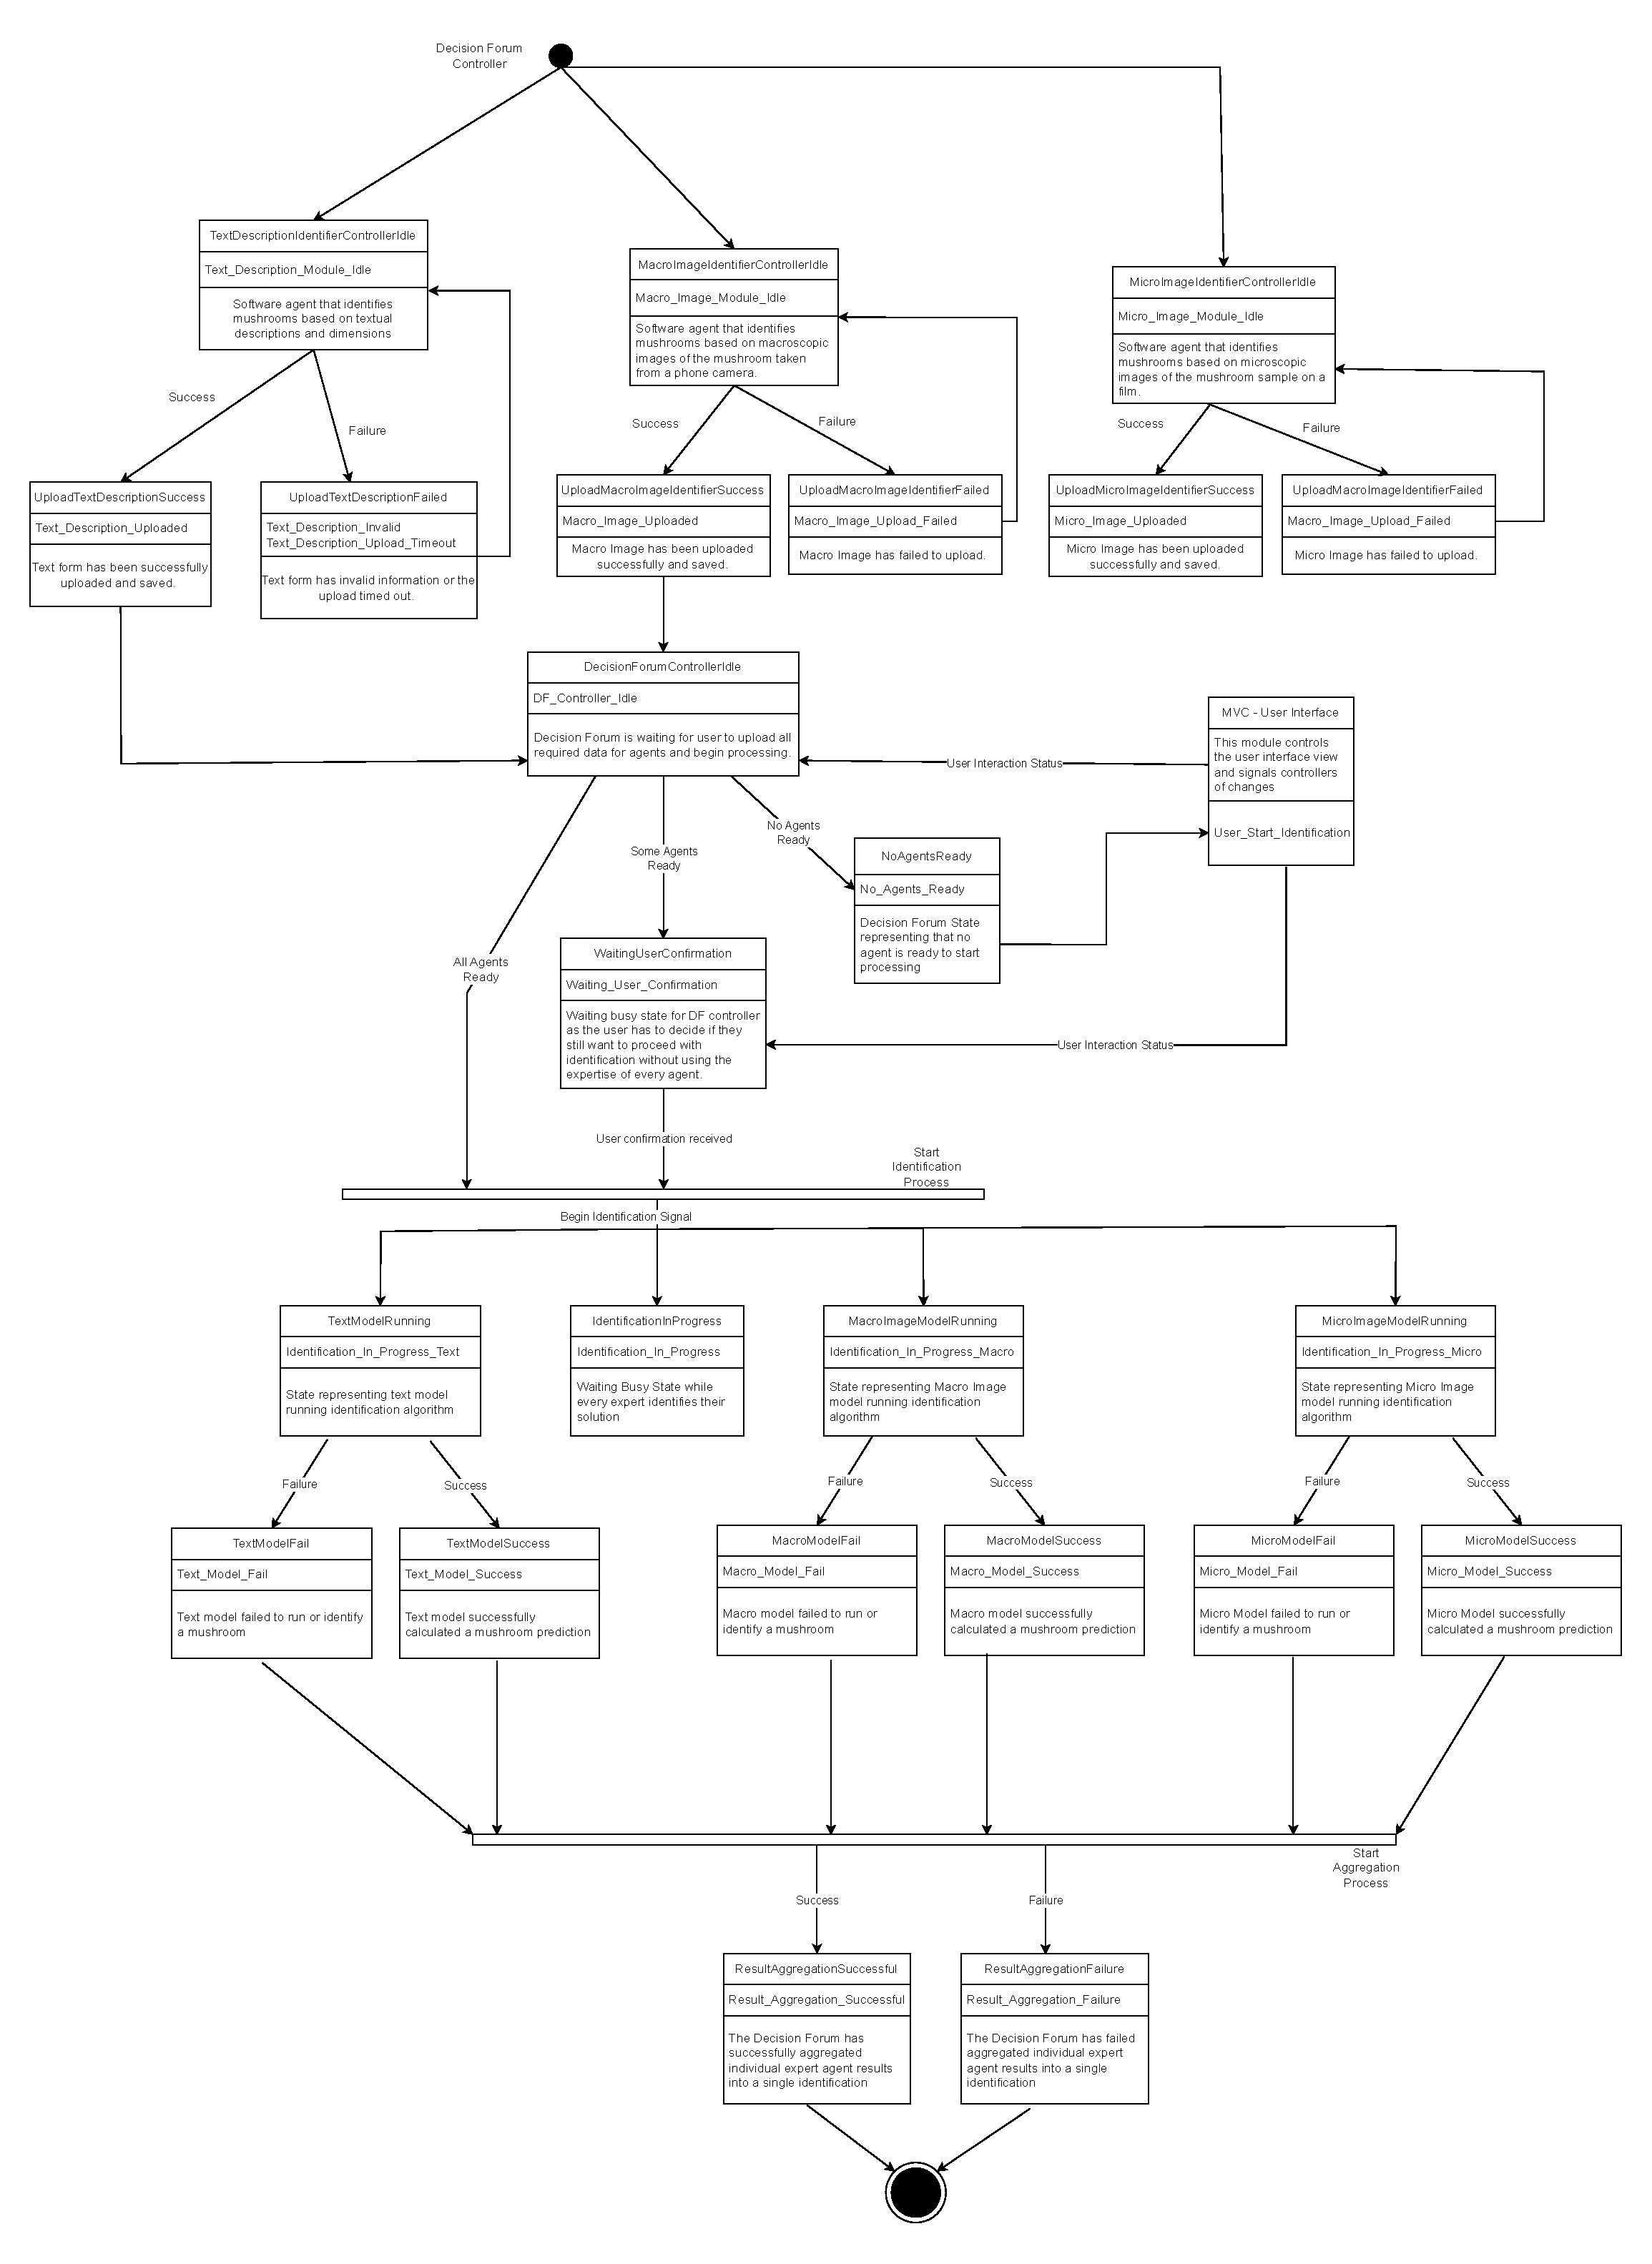
\includegraphics[width=0.9\textwidth]{SE3A04_D3_Diagram_Omar-Page-1.drawio.pdf}
    \caption{State Chart Diagram for the Decision Forum Controller}
\end{figure}

\begin{figure}[H]
    \centering
    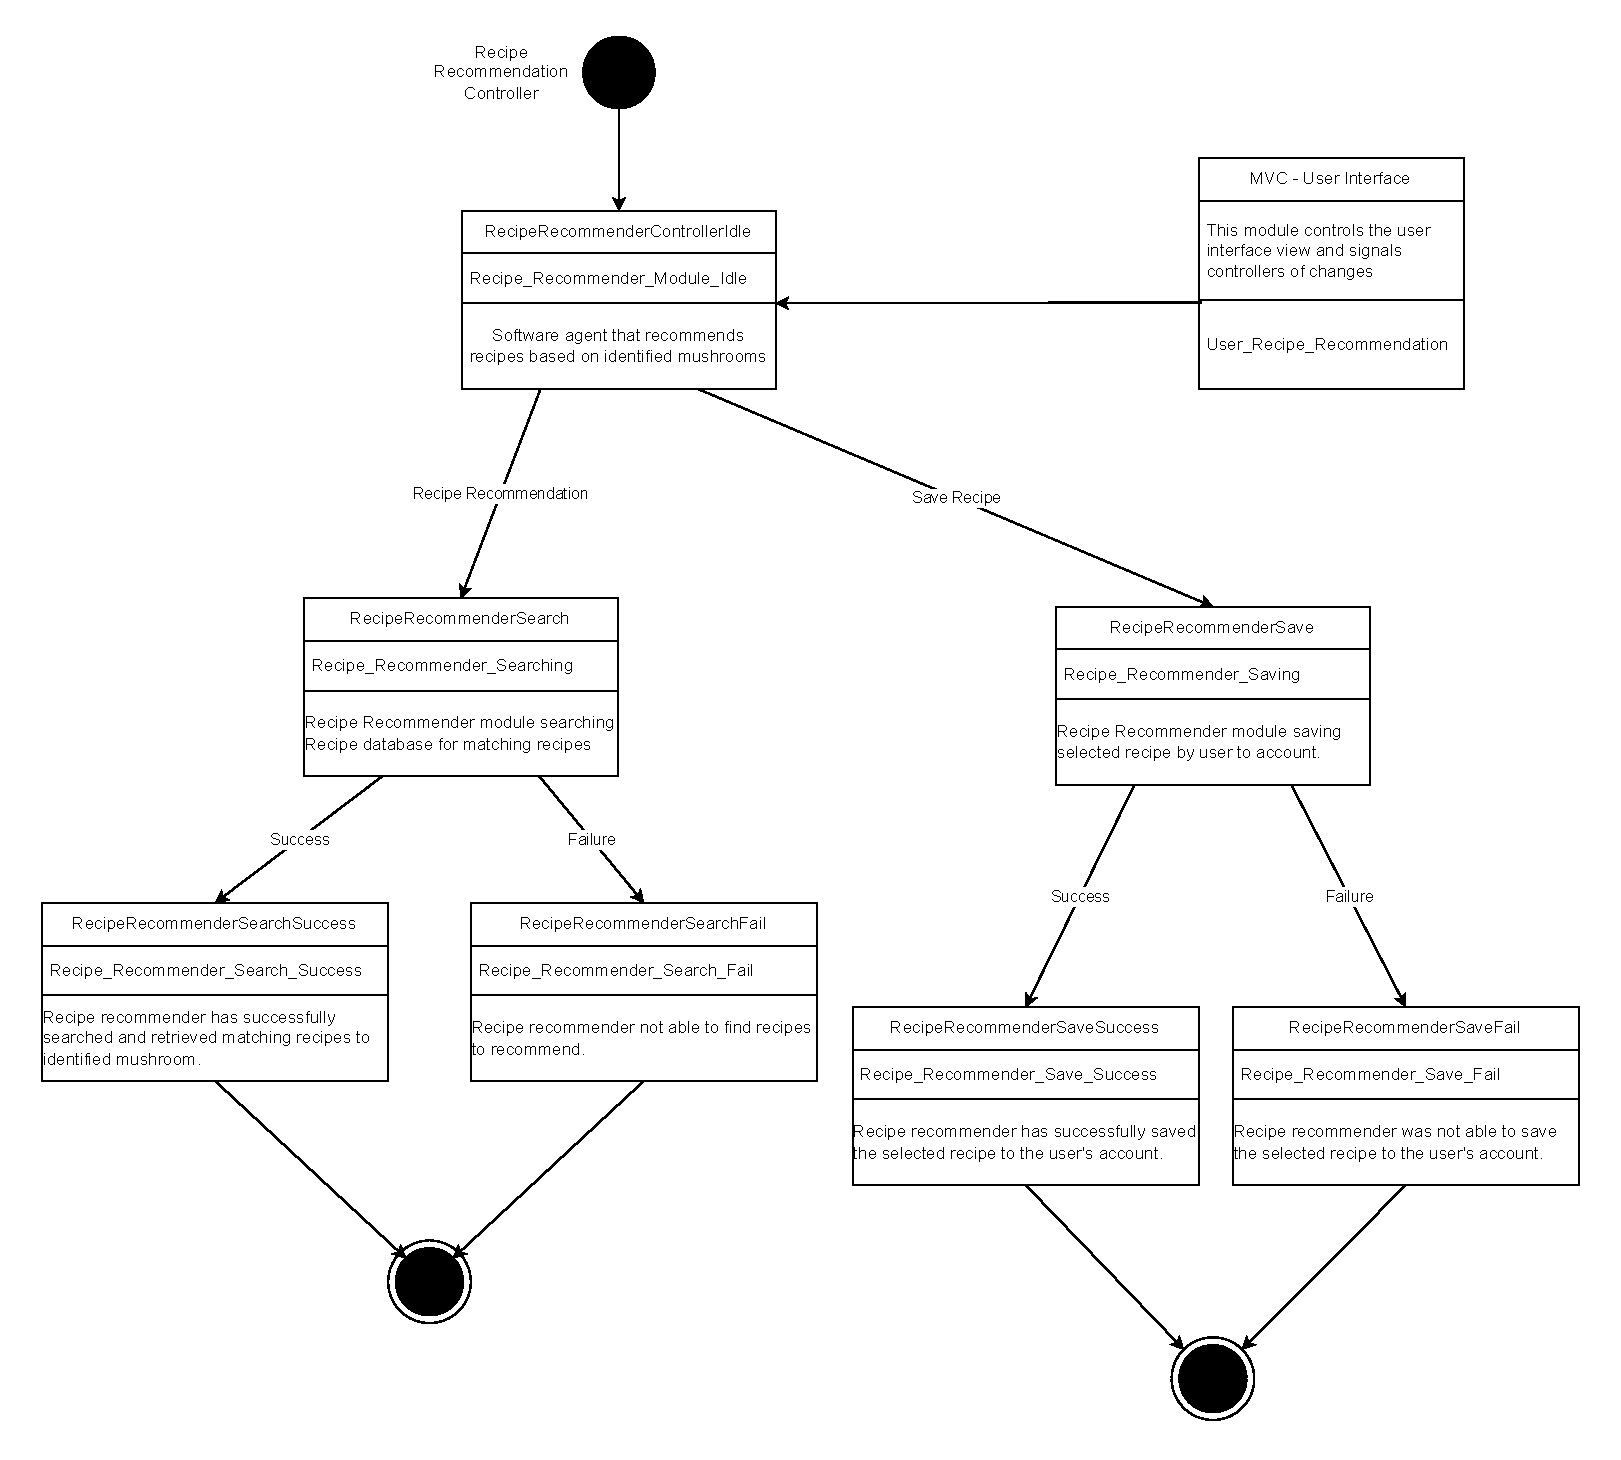
\includegraphics[width=\textwidth]{SE3A04_D3_Diagram_Omar-Page-2.drawio.pdf}
    \caption{State Chart Diagram for the Recipe Recommendation Controller}
\end{figure}

% \begin{figure}[h]
%     \centering
%     \includegraphics[width=\textwidth][height=\textheight]{SocialMediaStateDiagram.pdf}
%     \caption{PlantUML Diagram}
% \end{figure}

\begin{figure}[h]
    \centering
    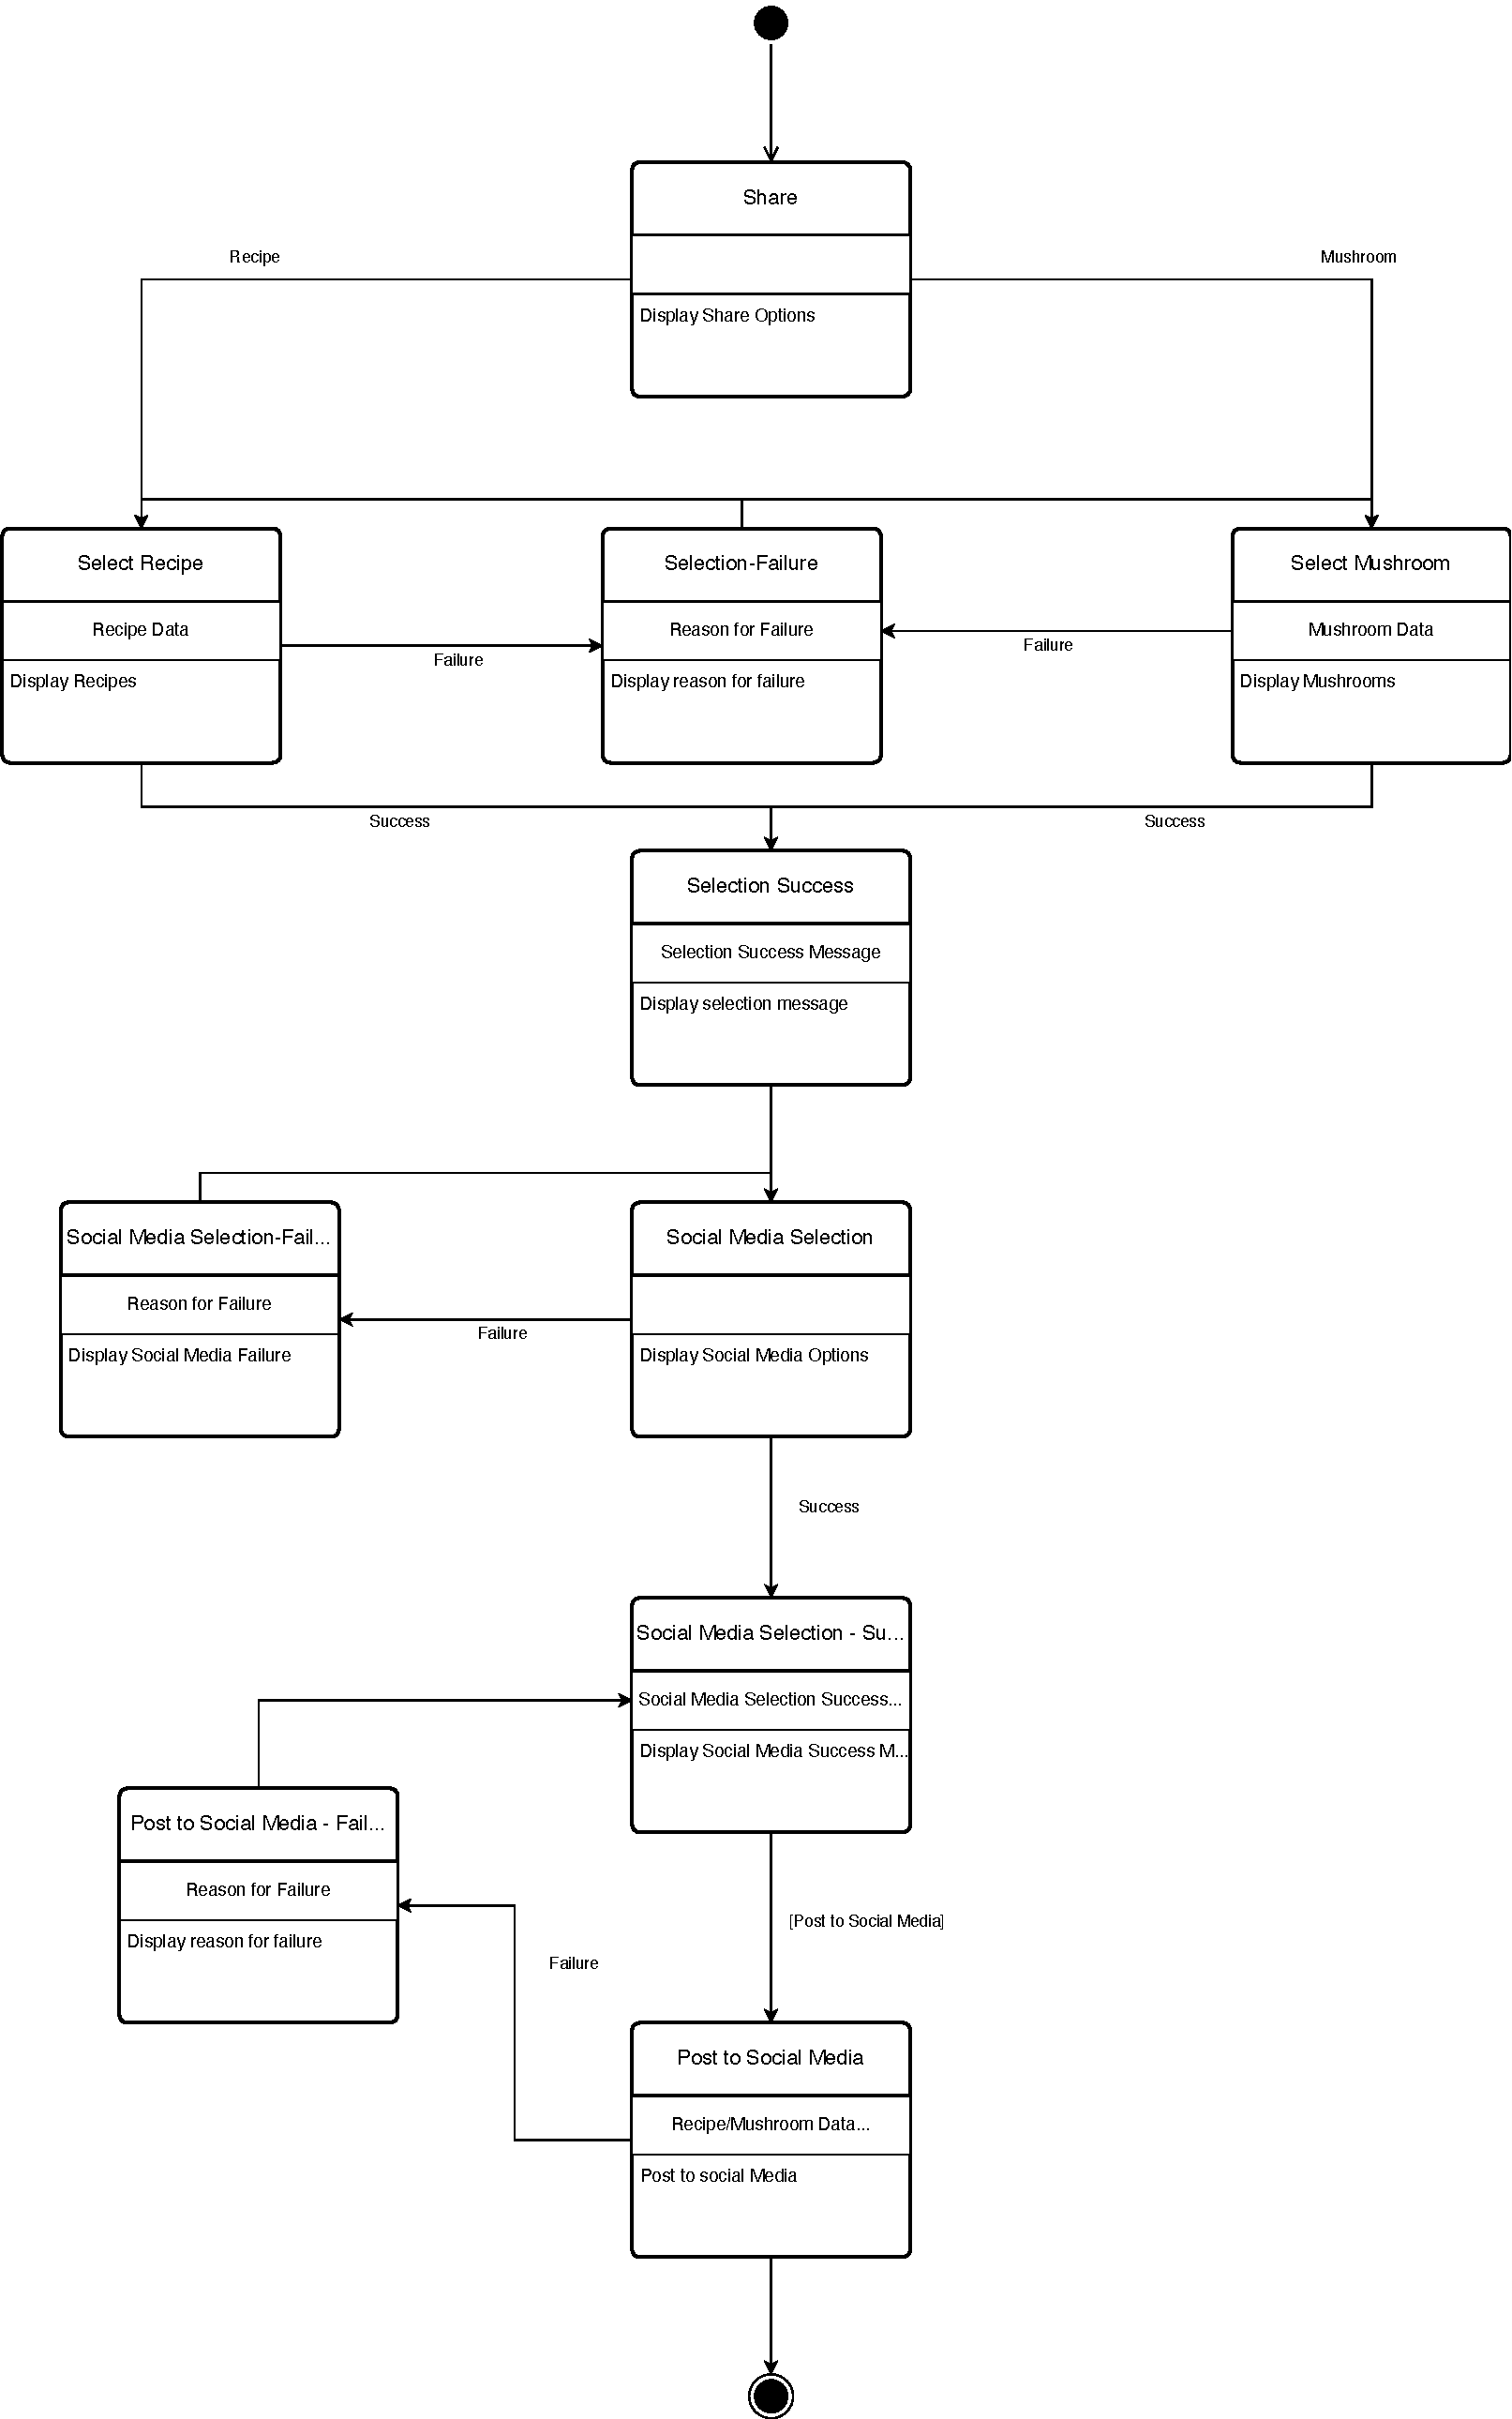
\includegraphics[width=\textwidth, height=0.9\textheight, keepaspectratio]{SocialMediaStateDiagram.pdf}
    \caption{State Chart Diagram for the Social Media Manager Controller}
\end{figure}

\clearpage

\begin{figure}[h]
    \centering
    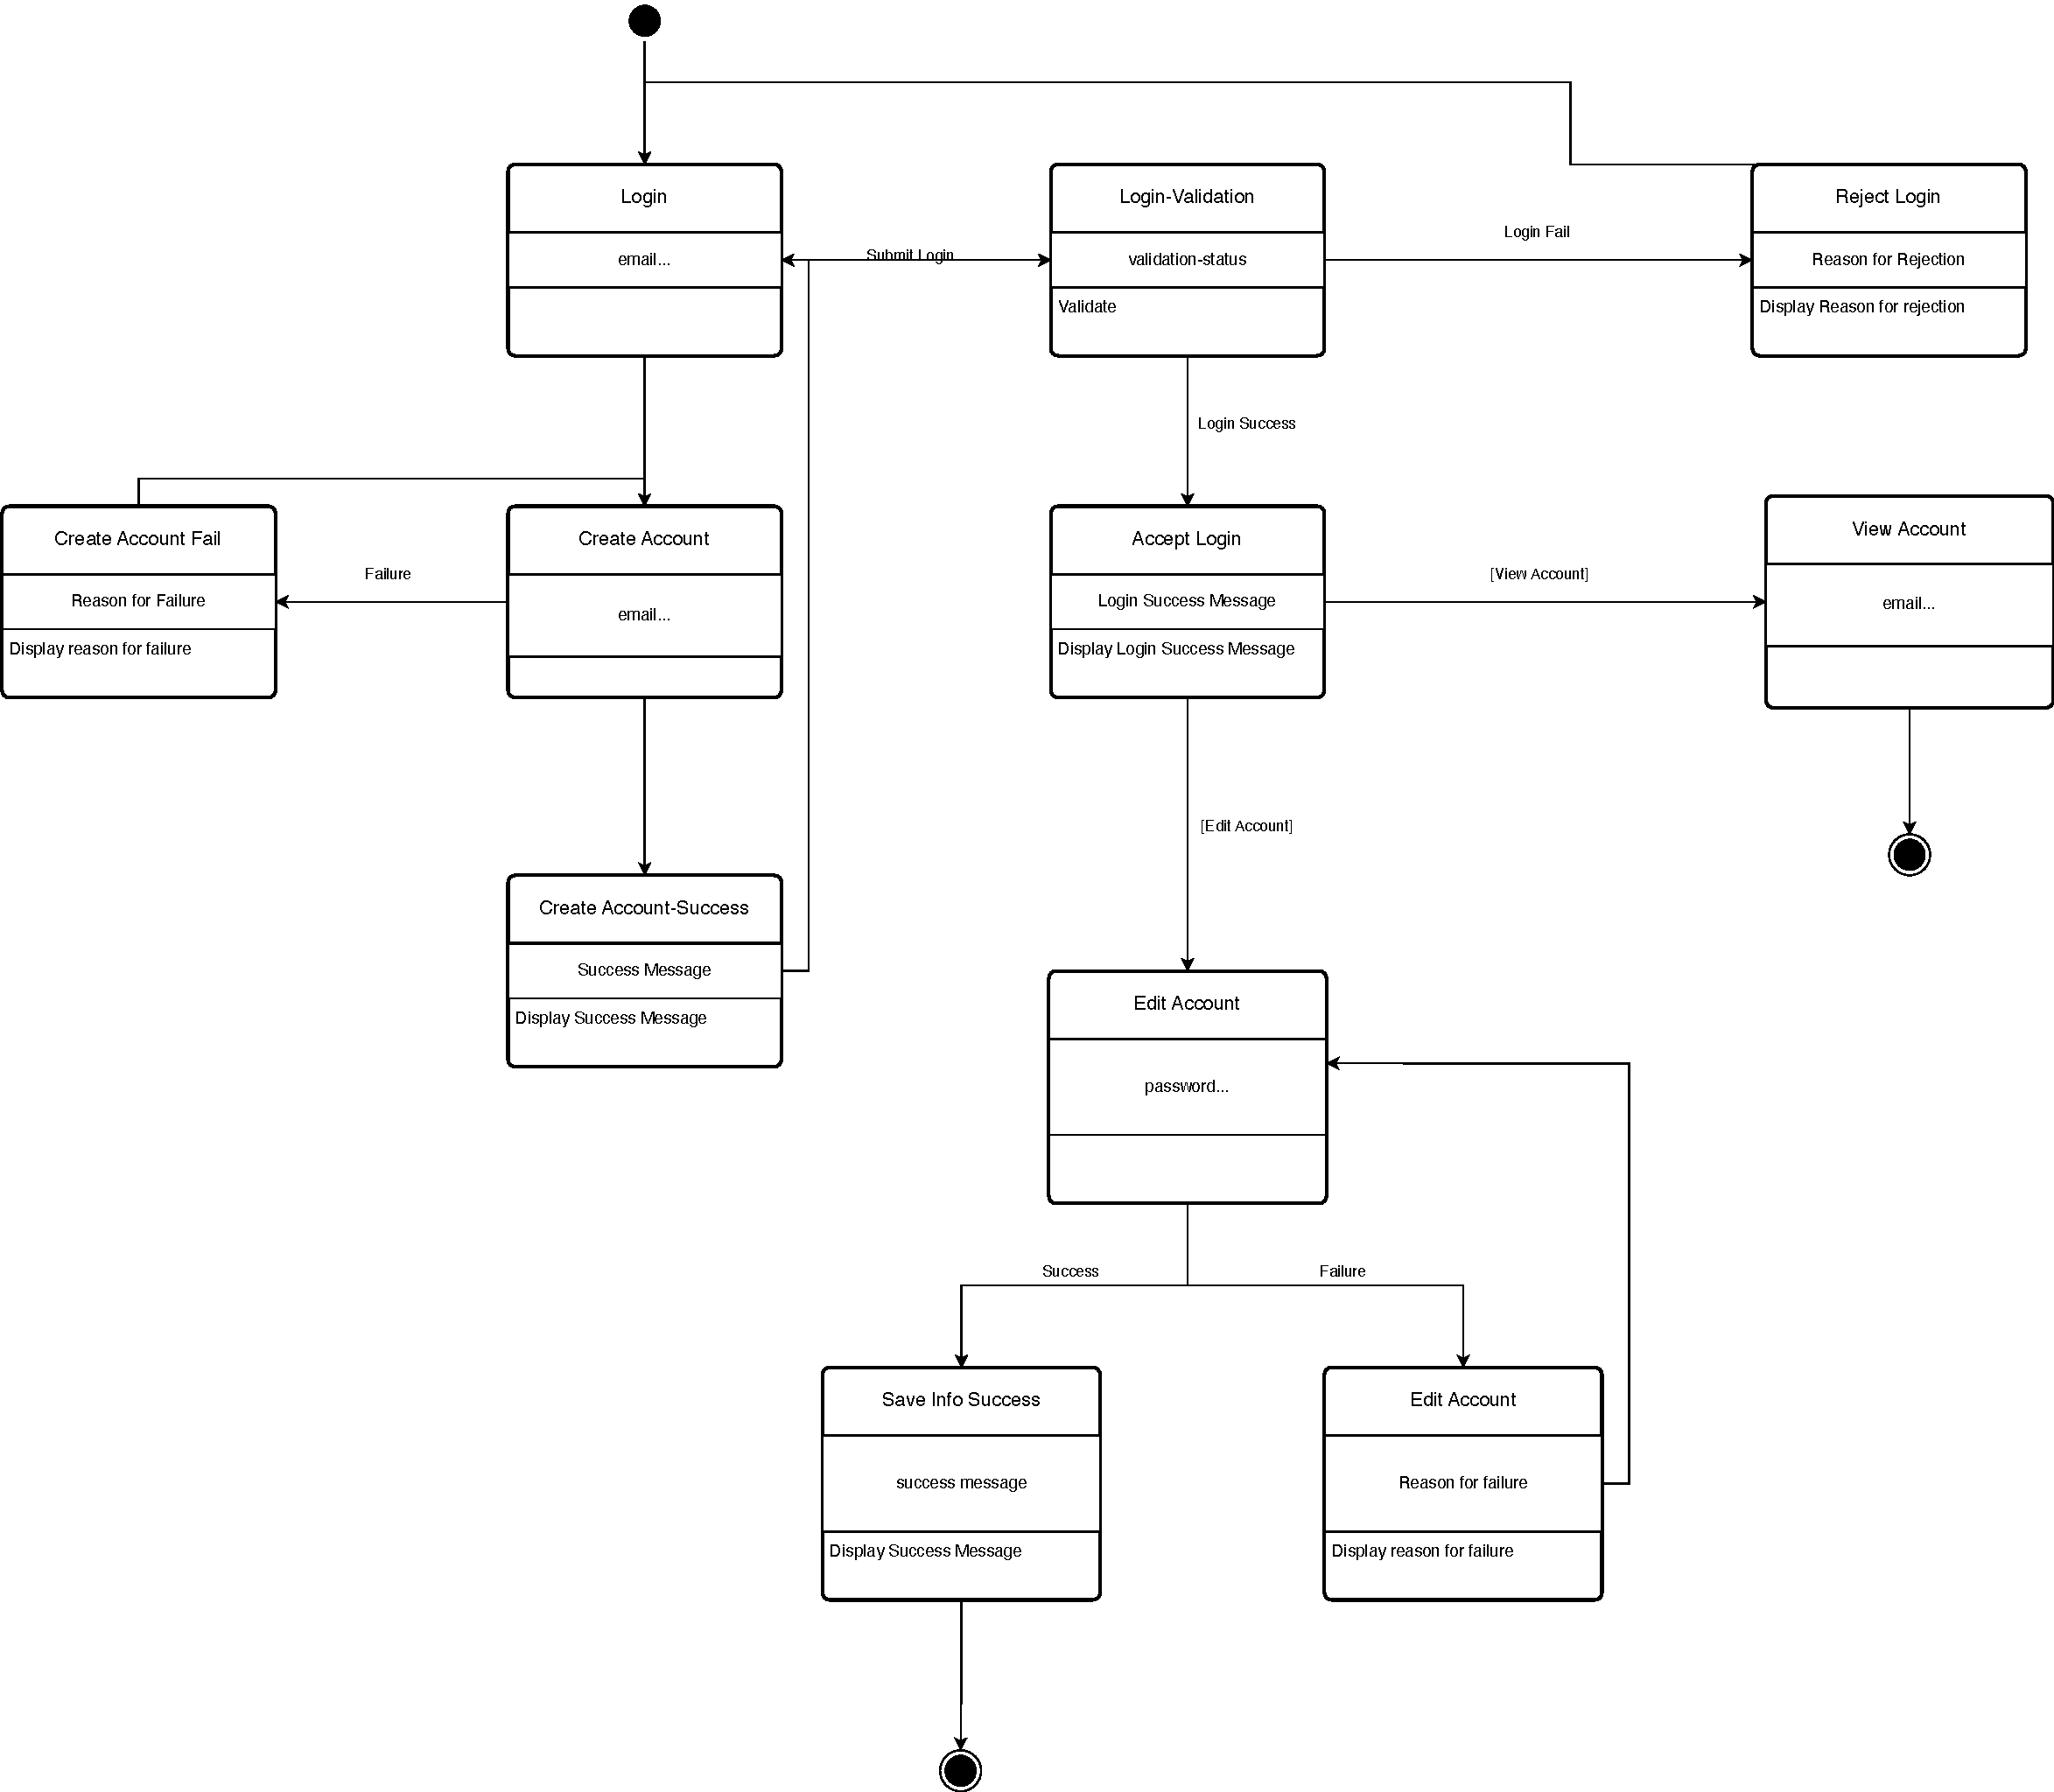
\includegraphics[width=\textwidth]{AccountStateDiagramFinal.pdf}
    \caption{State Chart Diagram for the Account Manager Controller}
\end{figure}

% End Section

\newpage

\section{Sequence Diagrams}
\label{sec:sequence_diagrams}
% Begin Section
% Register and Login Sequence Diagrams

\begin{figure}[H]
    \centering
    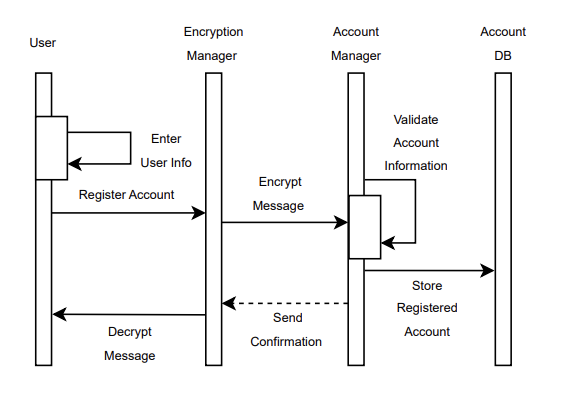
\includegraphics[width=0.77\textwidth]{RegisterSequenceDiagram.png}
    \caption{Register Account Sequence Diagram}
    \label{fig:register}
\end{figure}


\begin{figure}[H]
    \centering
    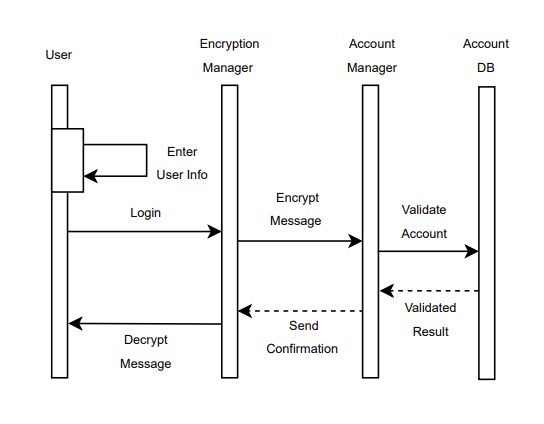
\includegraphics[width=0.77\textwidth]{LoginSequenceDiagram.png}
    \caption{Login Sequence Diagram}
    \label{fig:login}
\end{figure}

\begin{figure}[H]
    \centering
    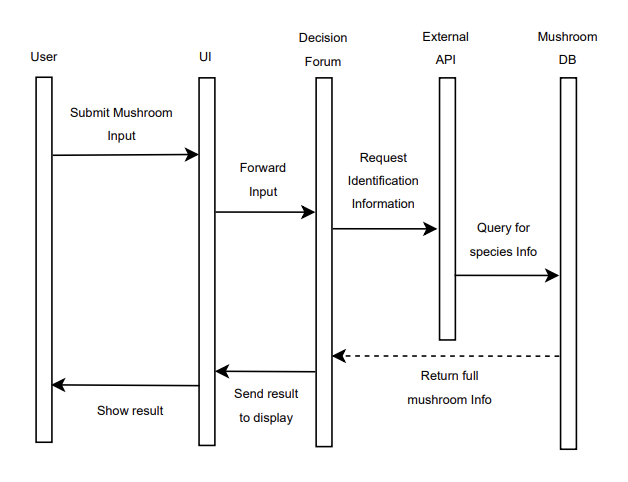
\includegraphics[width=0.8\textwidth]{IdentifyMushroomSequenceDiagram.png}
    \caption{Identify Mushroom Sequence Diagram}
    \label{fig:identify}
\end{figure}


\begin{figure}[H]
    \centering
    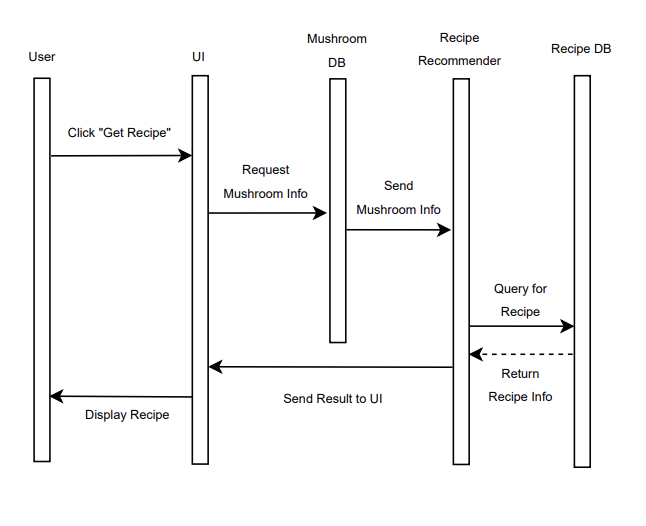
\includegraphics[width=0.76\textwidth]{GetRecipeSequenceDiagram.png}
    \caption{Get Recipe Sequence Diagram}
    \label{fig:recipe}
\end{figure}

\vspace{1.5cm}

\begin{figure}[H]
    \centering
    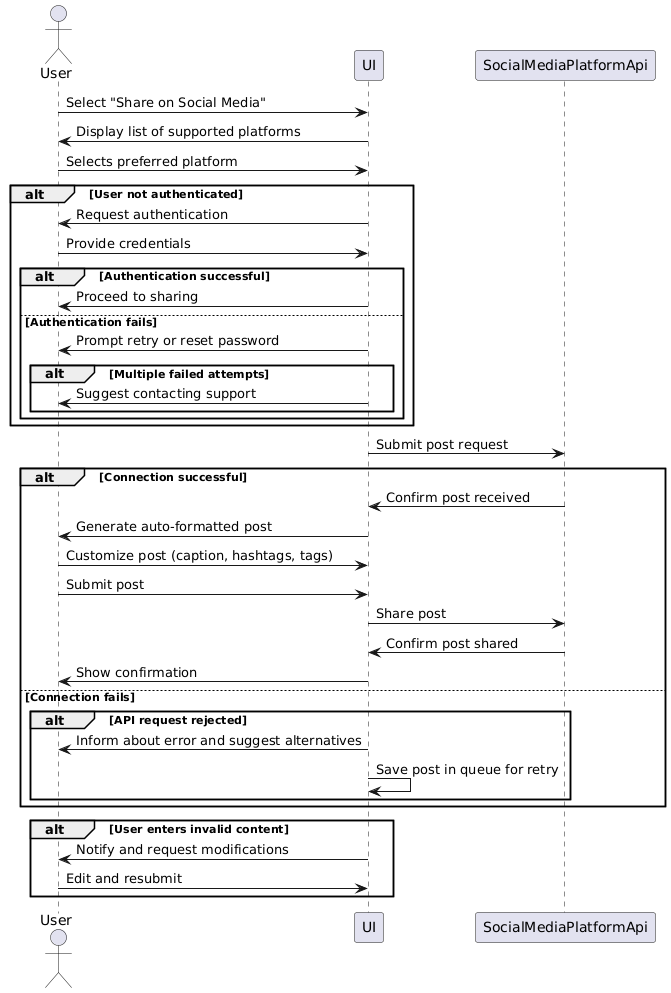
\includegraphics[width=0.82\textwidth]{sharetosocialmedia.png}
    \caption{Share to Social Media Diagram}
    \label{fig:identify}
\end{figure}

\vspace{0.4cm}

\begin{figure}[H]
    \centering
    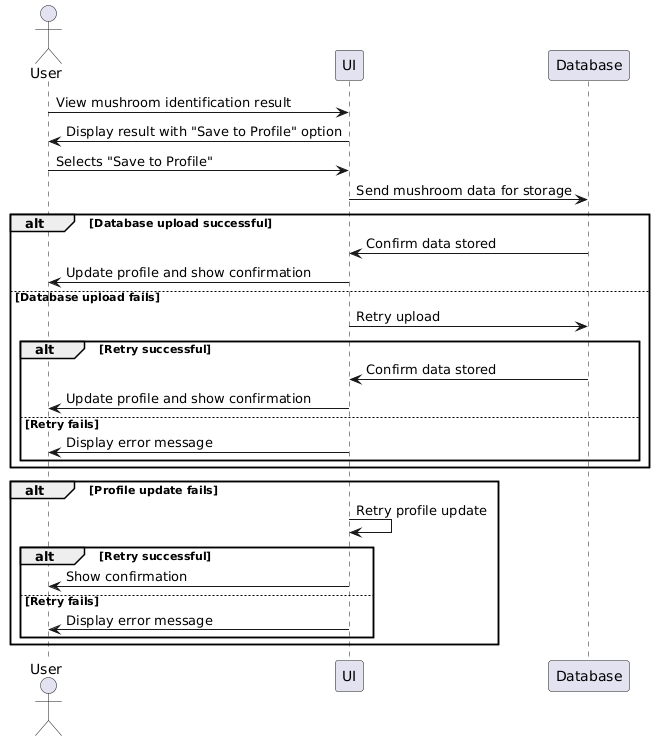
\includegraphics[width=0.82\textwidth]{savemushroom.png}
    \caption{Save Mushroom to Account Diagram}
    \label{fig:recipe}
\end{figure}


% End Section

\clearpage
\section{Detailed Class Diagram}
\label{sec:detailed_class_diagram}
% Begin Section
% This section should provide a detailed class diagram for your application.
The diagrams is provided as SVG file and may be zoomed into to reveal more detail.
\begin{figure}[h]
    \centering
    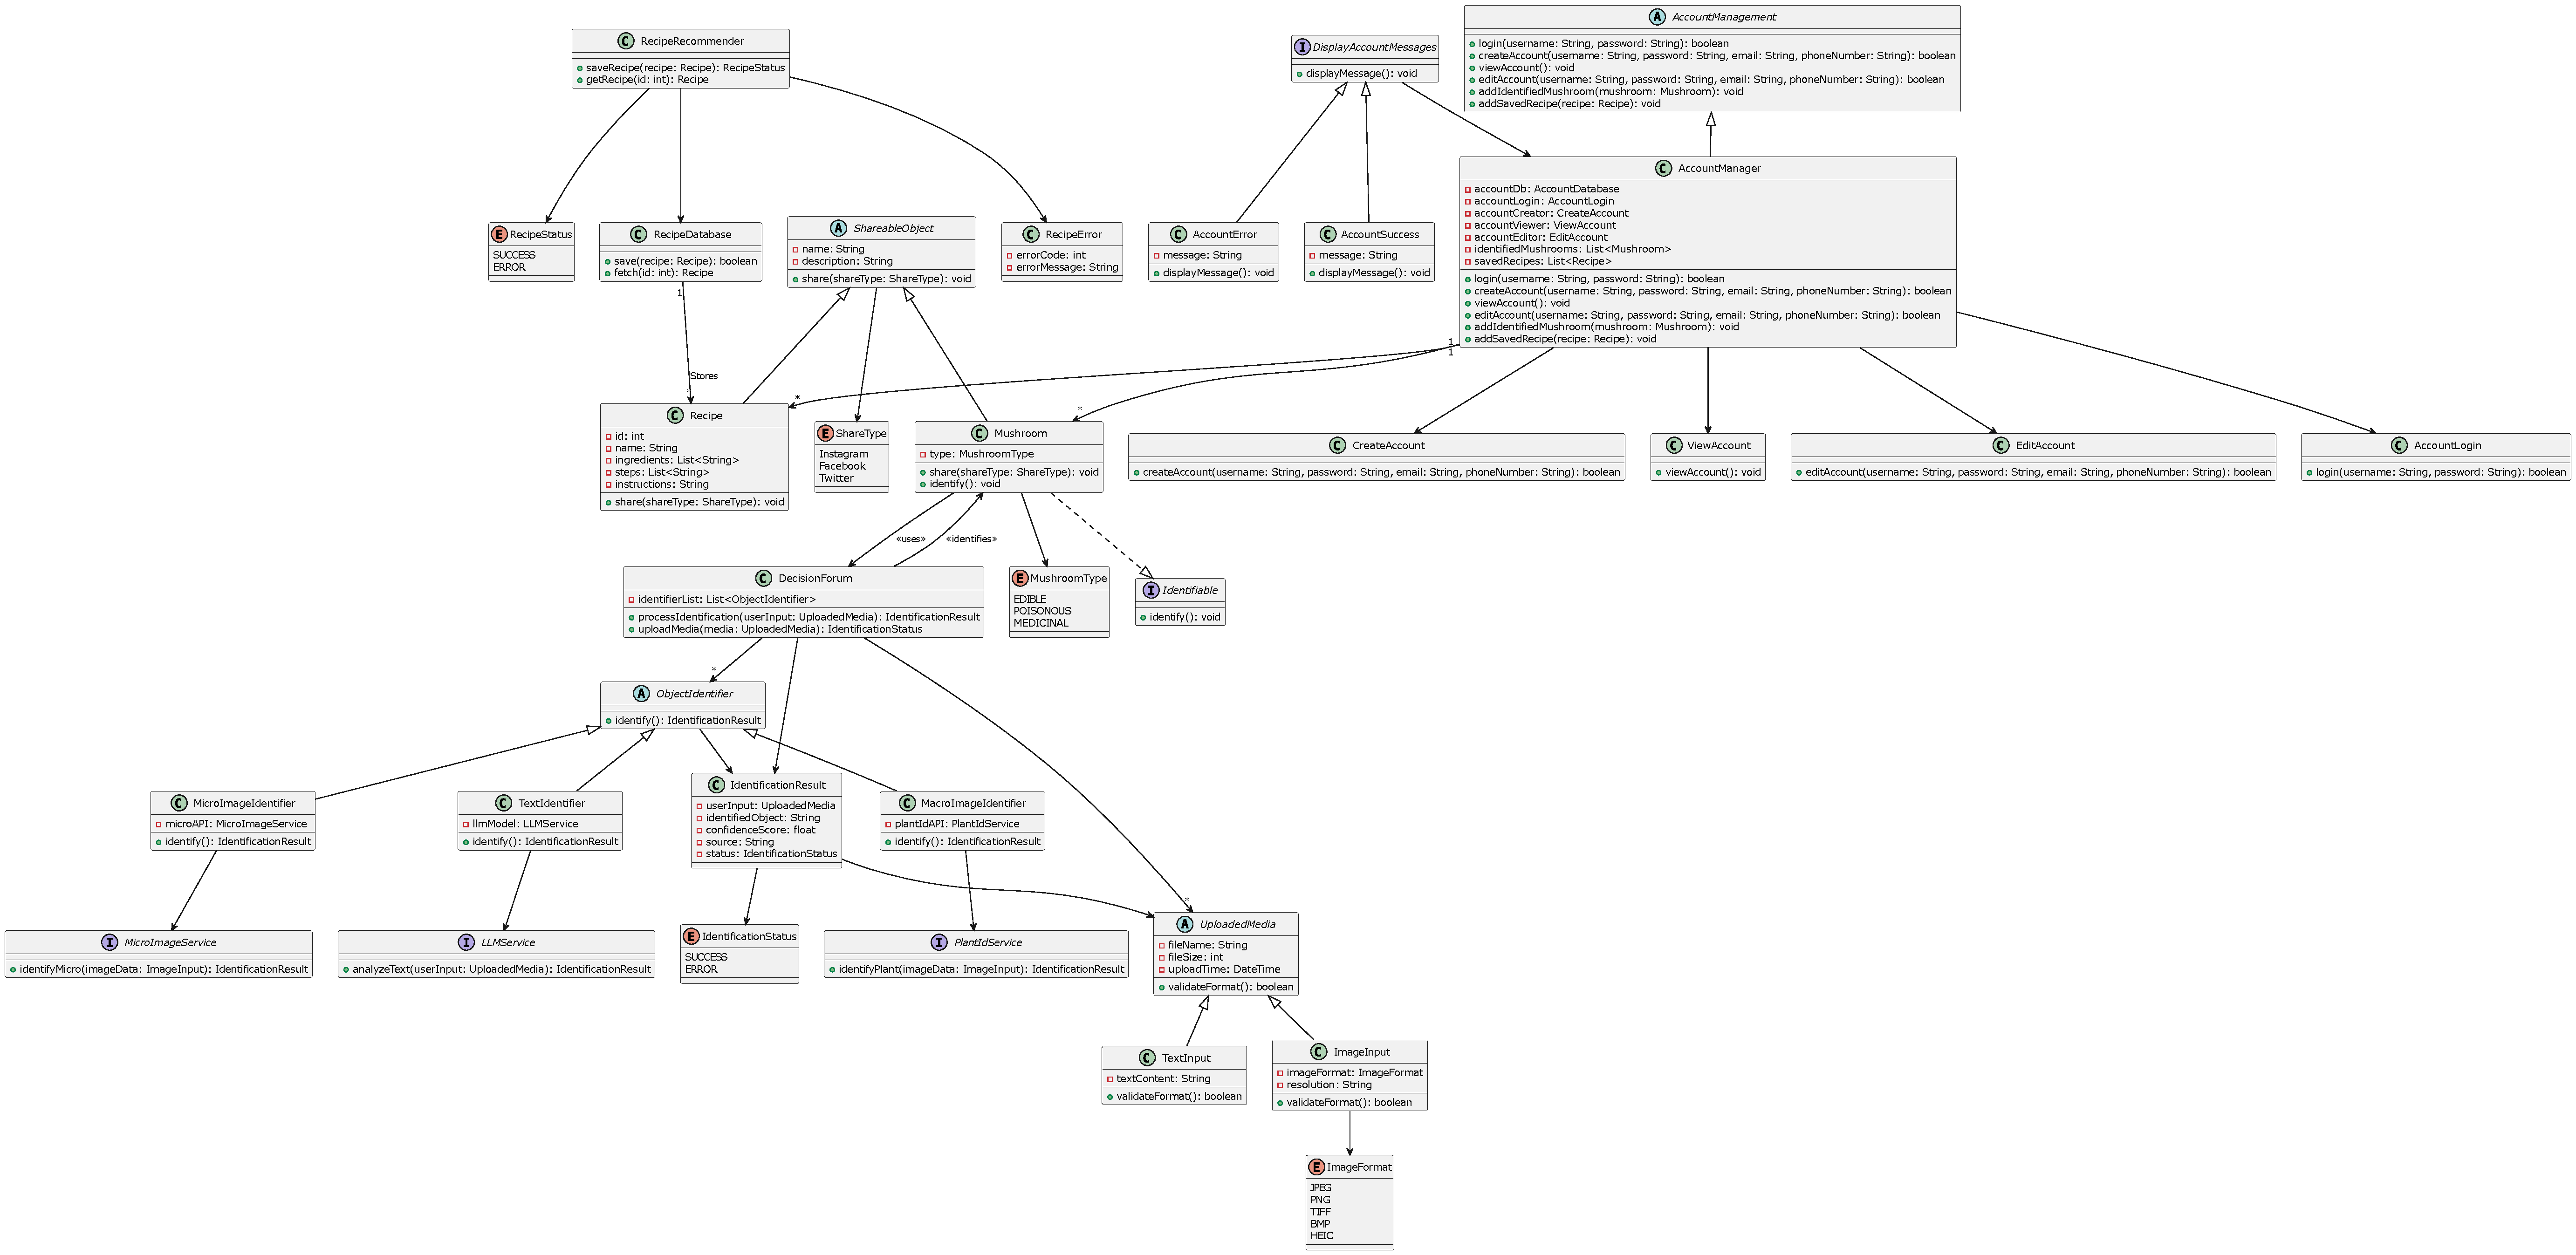
\includegraphics[width=\textwidth]{DetailedClassDiagramFinal.pdf}
    \caption{Detailed Class Diagram}
\end{figure}
% End Section

\clearpage
\appendix
\section{Division of Labour}
\label{sec:division_of_labour}
% Begin Section
Include a Division of Labour sheet which indicates the contributions of each team member. This sheet must be signed by all team members.
% End Section
% \begin{enumerate}
%     \item Omar Alam
%     \begin{itemize}
%         \item State chart diagrams for the Decision Forum Controller and Recipe Recommendation Controller.
%         \item Latex formatting and editing.
%     \end{itemize}
%     \begin{figure}[H]
%         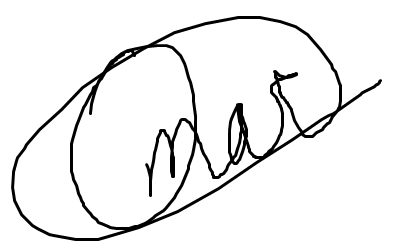
\includegraphics[scale=0.4]{omar-signature.png}
%     \end{figure}
% \end{enumerate}

\begin{itemize}
	% \item Include a Division of Labour sheet which indicates the contributions of each team member. This sheet must be signed by all team members.
	\item Farid Bastoros:
	\begin{itemize} 
		\item Section 4 - Detailed Class Diagram
	\end{itemize}
	
\includegraphics[scale=0.09]{Farid Bastoros - Signature.jpeg}\\ 
	\item Neha Bhatla:
	\begin{itemize} 
		\item 
	\end{itemize}
	
\includegraphics[scale=0.05]{neha_signature.jpeg}\\ 
	\item Omar Alam:
	\begin{itemize}
		\item State chart diagrams for the Decision Forum Controller and Recipe Recommendation Controller.
        \item Latex formatting and editing.
    
	\end{itemize}
	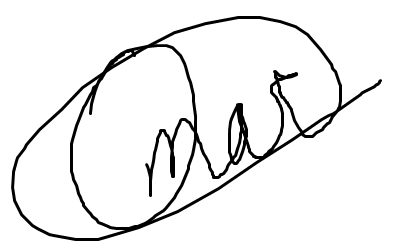
\includegraphics[scale=0.3]{omar-signature.png}\\
	% \item \begin{itemize} \end{itemize}
	\item Luka Mahrt-Smith:
	\begin{itemize}
		\item 
	\end{itemize} 
 	
\includegraphics[scale=0.1]{luka_signature.png}\\
	\item Aidan Lao:
	\begin{itemize} 
		\item 
	\end{itemize}
	
\includegraphics[scale=0.1]{aidan-signature.png}\\
	
	
\end{itemize}


\newpage



\end{document}
%------------------------------------------------------------------------------